\documentclass{article}


% if you need to pass options to natbib, use, e.g.:
%     \PassOptionsToPackage{numbers, compress}{natbib}
% before loading neurips_2022


% ready for submission
\usepackage{neurips_2022}


% to compile a preprint version, e.g., for submission to arXiv, add add the
% [preprint] option:
%     \usepackage[preprint]{neurips_2022}


% to compile a camera-ready version, add the [final] option, e.g.:
%     \usepackage[final]{neurips_2022}


% to avoid loading the natbib package, add option nonatbib:
%    \usepackage[nonatbib]{neurips_2022}


\usepackage[utf8]{inputenc} % allow utf-8 input
\usepackage[T1]{fontenc}    % use 8-bit T1 fonts
\usepackage{hyperref}       % hyperlinks
\usepackage{url}            % simple URL typesetting
\usepackage{booktabs}       % professional-quality tables
\usepackage{amsfonts}       % blackboard math symbols
\usepackage{nicefrac}       % compact symbols for 1/2, etc.
\usepackage{microtype}      % microtypography
\usepackage{xcolor}         % colors
\usepackage{amsmath,amssymb}
\usepackage{algorithm} 
\usepackage{algpseudocode} 
\usepackage{graphicx}
\usepackage{caption}
\usepackage{subcaption}
\usepackage{float}
\title{Latent Variable models for de-novo task learning}


% The \author macro works with any number of authors. There are two commands
% used to separate the names and addresses of multiple authors: \And and \AND.
%
% Using \And between authors leaves it to LaTeX to determine where to break the
% lines. Using \AND forces a line break at that point. So, if LaTeX puts 3 of 4
% authors names on the first line, and the last on the second line, try using
% \AND instead of \And before the third author name.

\author{%
  Yoel Sanchez Araujo\\
  Princeton Neuroscience Institute\\
  \texttt{sanchez.araujo@princeton.edu} \\
}

\begin{document}

\maketitle

\begin{abstract}
In this work we apply a variant of a Hidden Markov Model called the Input-Output HMM with input dependent emissions to learning data for one mouse. The data is neural data at two different time points in the task, stimulus presentation and reward delivery. This data is collected over a period of 19 training sessions while the mouse is acquiring the task. Sequential models such as HMM that contain latent states are prime for explaining the type of learning occurring in task acquisition. Our results demonstrate that we can pick up on 2 different states, engaged and dis-engaged, and that the period of time over which these states are more likely to be assumed correlates with task learning. We compare two different models of the HMM, corresponding to a different number of states. Results suggest that each model explains the two stages of data: stimulus and rewarded delivery better. Specially the two state model explains the stimulus period better and the 3-state model explains the reward delivery period better. 
\end{abstract}


\section{Introduction}
Understanding how the brain learns the abstract principles of a task is a fundamental challenge for neuroscience. This is a challenge on two fronts. First, from a scientific perspective this type of learning, from here on out called “task acquisition” has not been studied in detail. Rather, studies of learning focus on a period of time after a human or animal knows how to perform the task, and is thus learning about some additional manipulation that requires certain actions to be performed. From a methodological point of view, the tools commonly used in neuroscience are for studying single manipulations that don’t have longer time scale dependencies. For example, a neuroscientist might study how certain neurons fire when a mouse is presented with different visual stimuli. This is often done with a Generalized Linear Model (GLM). Then, if scientists want to look at multiple sessions worth of data they often either average the data, or fit a GLM independently for each session to estimate parameters of interest, such as the spiking rate in a Poisson GLM. Thus they are throwing away information about the evolution of the parameters they are estimating.  Recent lines of research have applied Hidden Markov models (HMM) to behavioral and neural data to try and predict animal behavior, given the animal is in a certain state, as estimated by the HMM. By leveraging HMMs in this way researchers have been able to explain behavior to a greater degree [1, 2, 3]. There has yet to be a work however, where an HMM is leveraged to explain neural data while an animal is acquiring a task de-novo. 

\noindent
The data we will use will come from mice performing a two alternative forced choice task. In this task a mouse sits on a platform with it's paws on a wheel, and a screen directly in front of the mouse. A visual stimulus appears on either the left or right side of the screen and the mouse must move the wheel such that it brings the visual stimulus to center of the screen. In this way the mouse is forced to make one of two choices (it must either move the wheel to the right or the left). Although technically the mouse can not perform an action at all, we are for the moment simplifying the behavior and task to a two-alternative forced choice one. We will have neural data from 3 regions in the brain that are associated with decision making and learning. Crucially, the neural and behavioral data collection will happen right when the mice are first exposed to the task. This is in contrast to most neuroscience work in mice, where they learn the structure of the task before any neural data is collected. 

\noindent
We will specifically use the HMM together with a GLM to form a input-output HMM (IO-HMM), a variant of [4]. The likelihood for the GLM will take the form of a Gaussian, and we will have input driven emissions. Our over-arching goal is to use the latent variable state to help explain the neural data in greater detail. For example, if we are looking at the periods in a task where the mouse is rewarded, typically we see a response in the brain. However, we expect that this response is different depending on whether the mouse is engaged or not. Clearly, if we have no way to segment the periods where the mouse is in these different states, then the averages of the neural data corresponding to reward will conflate both states and provide a less accurate representation of the brain response to reward. 

\section{Methods}
\subsection{Latent variable model}
An IO-HMM is interesting for understanding and chunking animal behavior in neuroscience because it allows for the additional aspect of supervised learning in an HMM. This would in theory help us explain relationships between the animal's behavior and task relevant stimuli that they must take into account and act on. In the section that follows we will outline our model: 

\def\Nk{N_{1:k}}
\def\Nkm1{N_{1:k-1}}
\def\Nkp1{N_{k+1:t}}
\def\Nkp2{N_{k+2:t}}
\def\Nm{N_{1:t}}


% mu
\def\Lk{L_{1:k}}
\def\Lkm1{L_{1:k-1}}
\def\Lkp1{L_{k+1:t}}
\def\Lkp2{L_{k+2:t}}
\def\Lm{L_{1:t}}
% theta_v
\def\xk{x_{1:k}}
\def\xkm1{x_{1:k-1}}
\def\xkp1{x_{k+1:t}}
\def\xkp2{x_{k+2:t}}
\def\xm{x_{1:t}}

\def\E{\mathbb{E}}

\paragraph{Notation \& derivation}
$\xm$ denotes the stimuli, or control variates. $\Lm$ denotes the set of latent variables.  $\Nm$ denotes the set of neural variables. The likelihoods $P(N | L, x)$ take the form of Gaussians.
We want the conditional distribution over the latent variables $\Lm$, that determines the dynamics of the neural data $\Nm$. This conditional is $P(\Lm | \Nm, \xm)$, using Bayes rule we have: 

\begin{equation}
        \begin{aligned}
        P(\Lm | \Nm, \xm) & \propto P(\Nm,| \Lm, \xm) \times P(\Lm ) \\ \\
        & = P(N_{k+1:t}, L_{k+1:t}, \Nk, \Lk | \xm) \\ \\
        & = \underbrace{P(N_{k+1:t}, L_{k+1:t}| L_k, \xm)}_\text{backward} \times \underbrace{P(\Nk, \Lk | \xm)}_\text{forward}
        \end{aligned}
\end{equation}

\noindent
because $L$ has finite and typically small support over the integers, we can easily find the normalizing constant needed for equality in (1). We can first layout the recursive form to be used for the forward algorithm, of all random variables for the following graphical model. The joint distribution of the random variables given the observed is: $P(\Nk, \Lk | \xm)$, which can be factored in the following way, using conditional independence properties that can be read out from the graph in figure 1: 

\begin{figure}[H]
  \centering
  \includegraphics[width=6cm]{graph_mod.png}
  \caption{Graphical model of the IO-HMM. Only 2 time steps are shown. $N$ is the neural data, $x$ are the inputs, such as what choice the mouse made, whether it was rewarded, and the stimulus that appeared on the screen. $L$ are the latent states. }
\end{figure}

\begin{equation}
    P(N_k | L_k, x_k) \times P(L_k | L_{k-1}) \times P(\Nkm1, \Lkm1 | \xm)
\end{equation}

\noindent
this allows us to write the following recursions for the $\alpha$ (forward) and $\beta$ terms in the forward-backward algorithm, firs the forward term:

\begin{equation}
     \alpha_{k}(L_k) = P(N_k | L_k, x_k) \times \sum_{l \in L_{k-1}} P(L_k | L_{k-1}) \times \alpha_{k-1}(L_{k-1})
\end{equation}

\noindent
and for the backwards term:
 
 \begin{equation}
    \beta_k(L_k) =  \sum_{l \in L_{k+1}}P(L_{k+1} | L_k)  \times P(N_{k+1} | L_{k+1}, x_{k+1}) \times \beta_{k+1}(L_{k+1})
\end{equation}


\subsection{Inference}
To estimate the variables of interest in this model we use expectation maximization (EM). We run 50 iterations maximum of the E-step, M-step alternations as going beyond this would not lead to improvements in terms of log-likelihood.  During the E-step we run the forward backward algorithm to get the $\alpha$ and $\beta$ terms in equatinos (3) and (4). With these we can compute the probability of being in a state $z_i$ at any time step $k$ as: 

\begin{equation}
    \boldsymbol{\gamma}(L_i) = \frac{\boldsymbol{\alpha}(L_i) \boldsymbol{\beta}(L_i)}{P(\boldsymbol{X})}
\end{equation}

\noindent
and the probability of adjacent state pairs as:

\begin{equation}
    \xi(L_{k-1}, L_k) = \frac{\alpha_k(L_{k-1})P(N_k | L_k, x_k)P(L_k | L_{k-1})\beta_k(L_k)}{P(\boldsymbol{X})}
\end{equation}

\noindent
during the M-step we compute the state-to-state transition matrix $A$ from $\xi(L_{k-1}, L_k)$, and the initial transition $\pi$ (time step 1) from $\gamma$:

\begin{equation}
    \pi_i = \frac{\gamma(L_{1, i})}{\sum_{i=1}^M \gamma(L_{1, i})}
\end{equation}

\begin{equation}
    A_{k, i} = \frac{\sum_{k=2}^N \xi(L_{k-1, i}, L_{k, i})}{\sum_{l=1}^M \sum_{k=2}^N \xi(L_{k-1, i}, L_{k, l})}
\end{equation}

\noindent
finally we estimate the set of weights $\boldsymbol{W}$, as a $(P \times M)$ matrix, where $M$ is the number of states, and $P$ is the length of the inputs $x$ and $\boldsymbol{n}$ is the vector of neural data. For each state $i \in [1:M]$: 
\begin{equation}
 \begin{aligned}
    p(L) = \frac{\boldsymbol{\gamma}(L_i)}{\sum_{k=1}^N \boldsymbol{\gamma}(L_{k, i})} \\ 
    \boldsymbol{P}_{i} = Diag(p(L))\\
    \boldsymbol{w}_i = \Big(\boldsymbol{X}^{\top} \boldsymbol{P}_{i} \boldsymbol{X}^{\top} \Big)^{-1}\boldsymbol{X}^{\top}\boldsymbol{P}_{i}\boldsymbol{n}
\end{aligned}
\end{equation}
\noindent
and from these the standard deviations: 
\begin{equation}
 \begin{aligned}
     \mu_i = \boldsymbol{X} \boldsymbol{w}_i \\ 
     \sigma_i = \frac{\boldsymbol{\gamma}(L_i)^{\top} \big(\boldsymbol{n} - \mu_i \big)^2}{\sum_{t=1}^N \gamma(L_{t, i})}\\
\end{aligned}
\end{equation}

this gives us the following algorithm for inference: 

\begin{algorithm}
	\caption{EM for IO-HMM} 
	\begin{algorithmic}[1]
		\For {$t,\ldots, max iteration$}
			    \State E-step: compute $\alpha$, $\beta$, $\xi$, $\gamma$ with equations 5 to 6
			    \State M-step: estimate $\pi$, $A$, $\boldsymbol{W}$, $\sigma$ with equations 7 to 10
			    \State update $\pi$, $A$, $\boldsymbol{W}$, $\sigma$
			    \State compute likelihoods with updated quantities
			    \State check log-likelihood for convergence
		\EndFor
	\end{algorithmic} 
\end{algorithm}

\section{Results}
\label{gen_inst}

Now we apply the IO-HMM to the neural data. The data consists of calcium signals from the nucleus accumbens core (NACC) as the mouse was acquiring the task. Roughly there are 80 to 100 thousand samples per session of training. Within each session there are a set of "trials" which denote periods where the animal sees a stimulus and makes a choice. We average the data within those trials into two different parts. The period between the stimulus appears, and the action is made. And the period between feedback and 0.5 seconds afterwards. This means we fit the data twice once on $\boldsymbol{n}_{stimulus}$ and another on $\boldsymbol{n}_{feedback}$. One of the challenges to fitting these models is deciding how many latent states the animals can be in. We only compare a 2 and 3 state model in terms of log-likelihood. Perhaps not surprisingly, each period of the task, stimulus deliver and reward presentation is better fit by a different number of states. In particular, at stimulus time the 2-state model has better log-likelihood. While at reward time the 3-state model has better log-likelihood, as shown in figure 2. 

\begin{figure}[H]
    \centering
    \subfloat[Stimulus presentation]{
        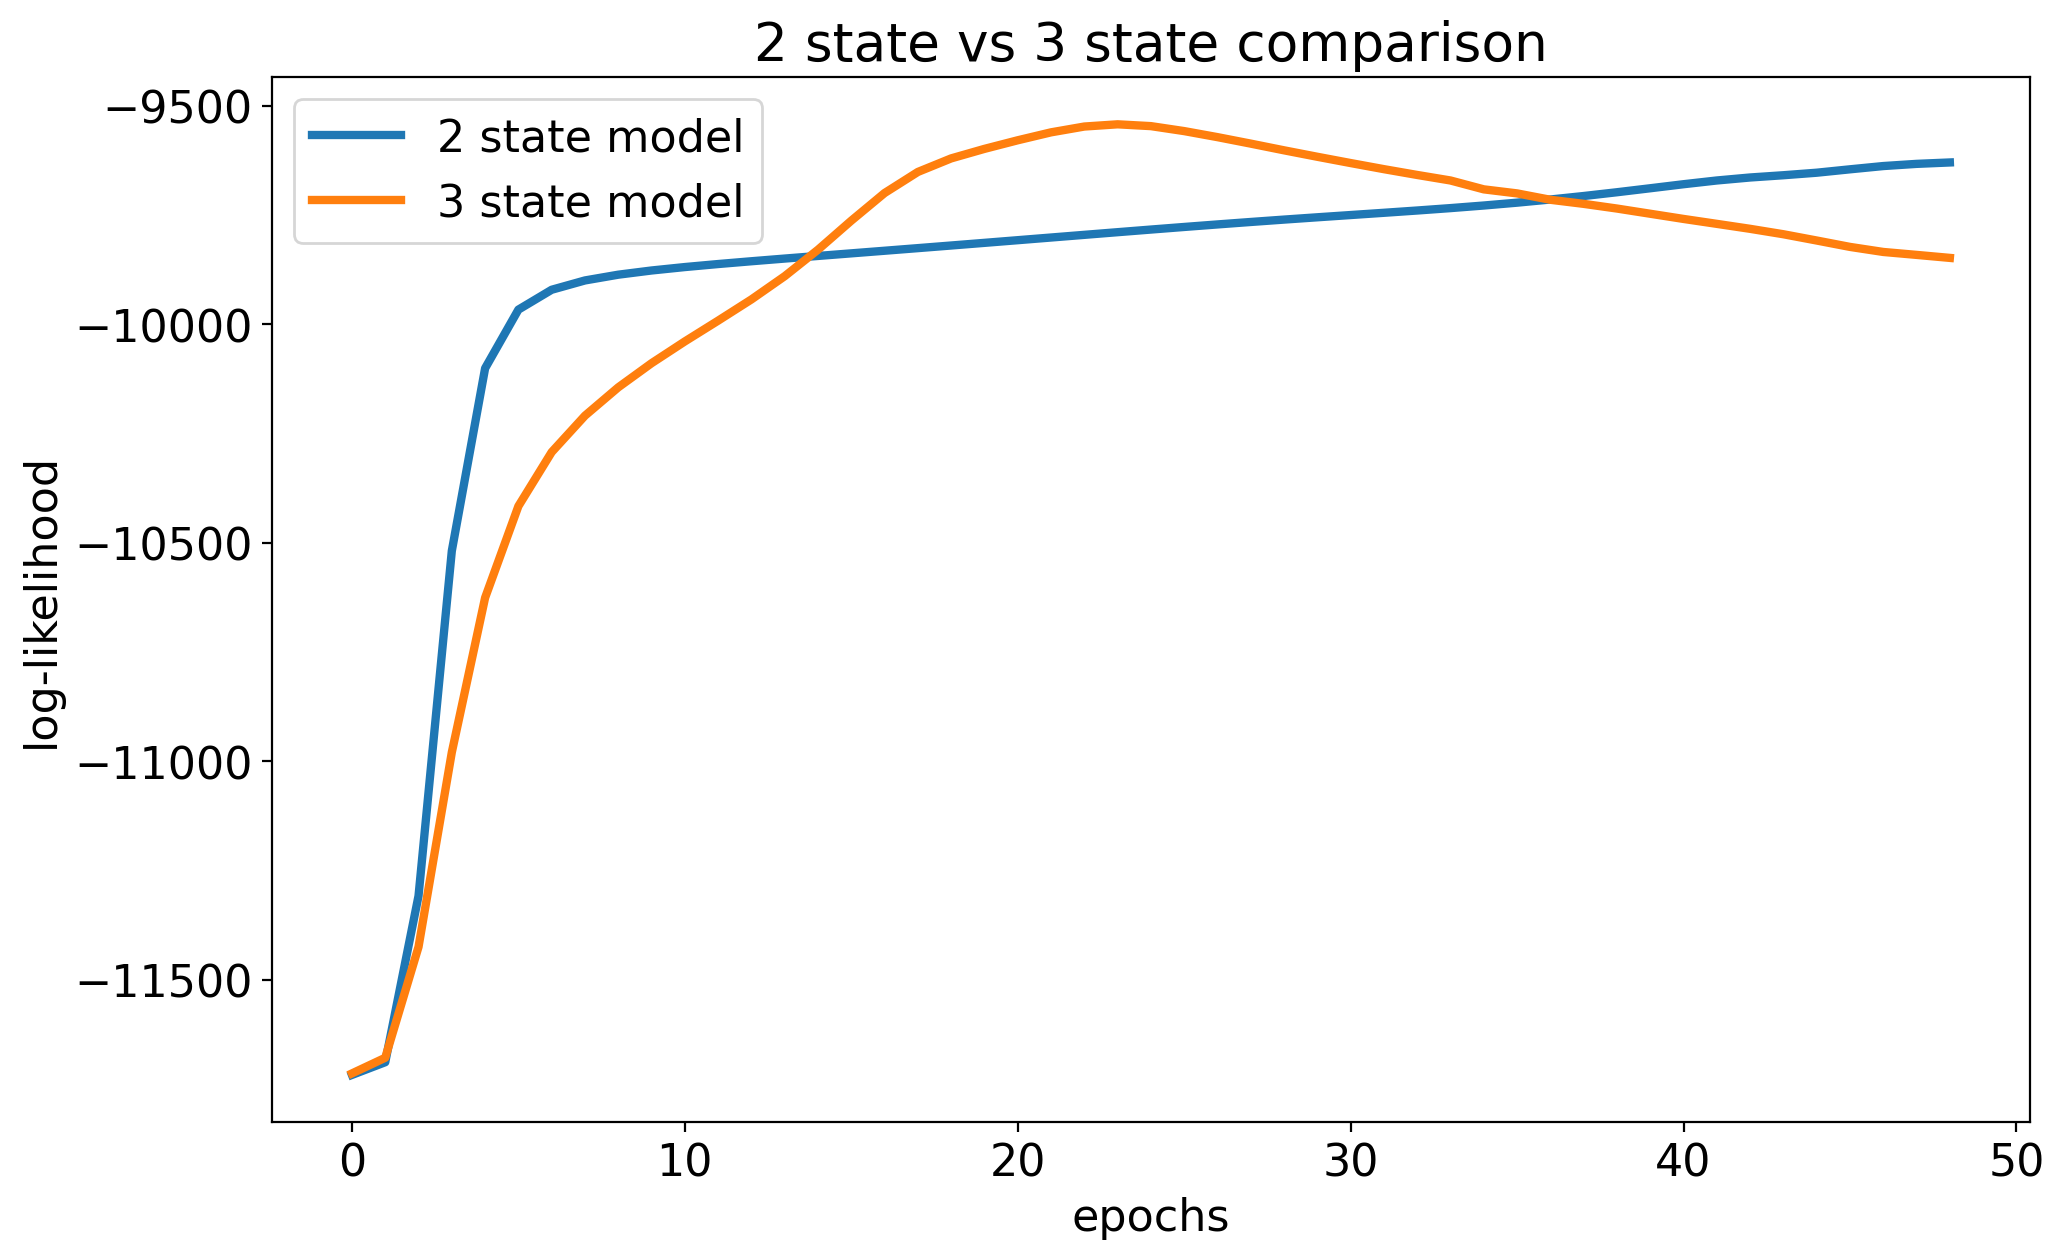
\includegraphics[width=0.55\textwidth] {stim_images/2state_vs3state_ll.png}
        \label{fig:Stimulus presentation} } \hspace*{-0.9em}
    \subfloat[Feedback period]{
        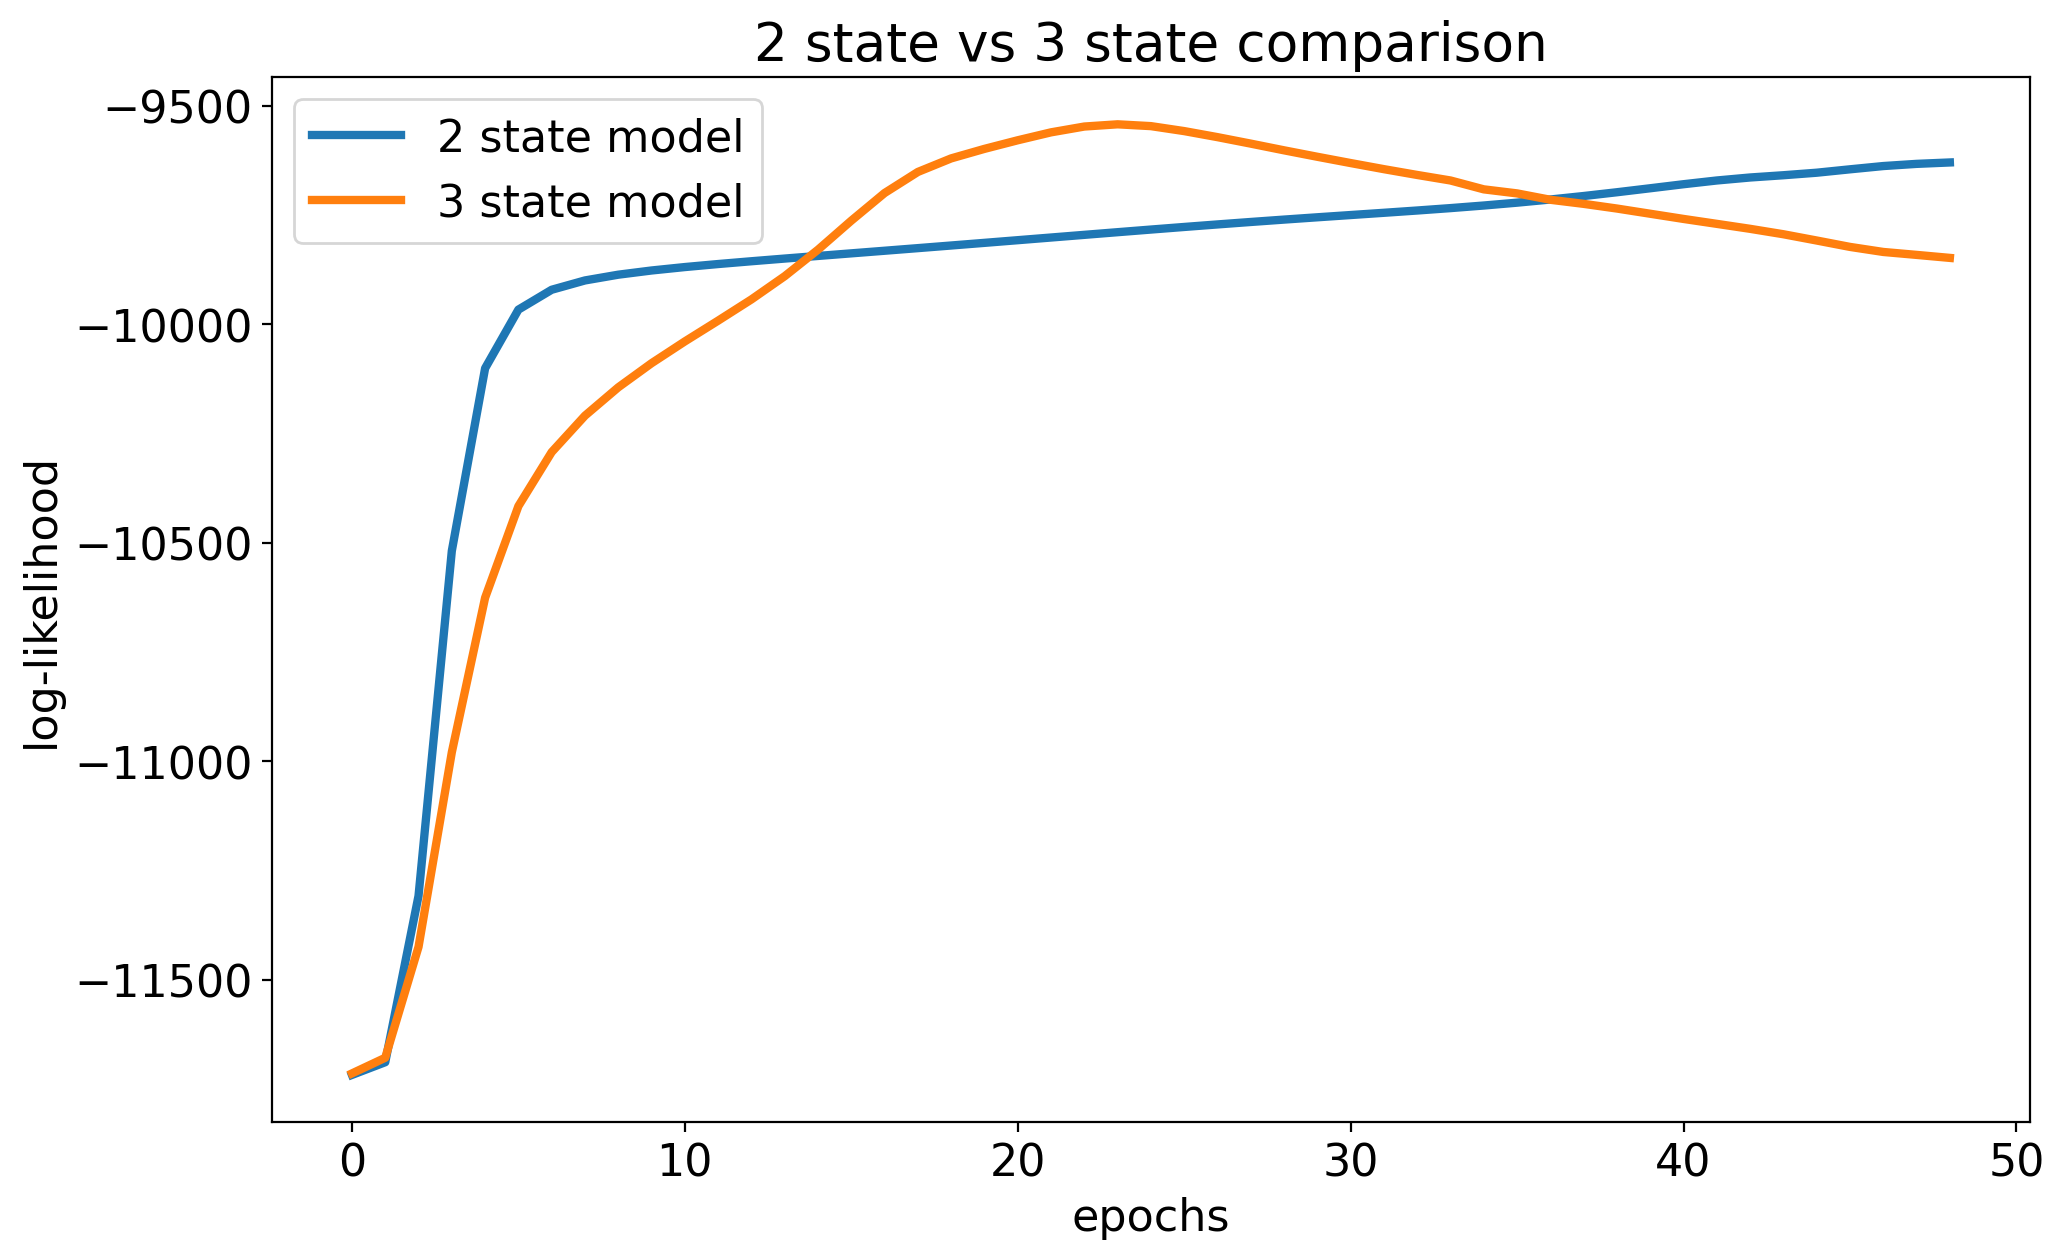
\includegraphics[width=0.55\textwidth] {stim_images/2state_vs3state_ll.png}
        \label{fig:feedback period}} \\
    \caption{Two state vs three state model comparison in terms of log-likelihood as optimizing occurred at stimulus presentation.}
\end{figure}
Next we investigate what the estimated weights are for the input driven emissions for the 2-state model at stimulus time. The inputs consisted of a matrix, where each row denoted a trial, and contained a total of 10 columns. The columns were: the choice the animal made, weather it was rewarded based on it's choice. And lastly 8 columns for the stimulus that appeared. The stimulus can appear on either the right or left side of the screen, at 4 levels of contrast. Therefor, if the stimulus appeared on the right side, at 25 percent contrast, on trial $t$, then the column for 25 percent contrast and stimulus on the right, in row $t$ contains a 1 and 0 otherwise. 
\begin{figure}[H]
\centering
 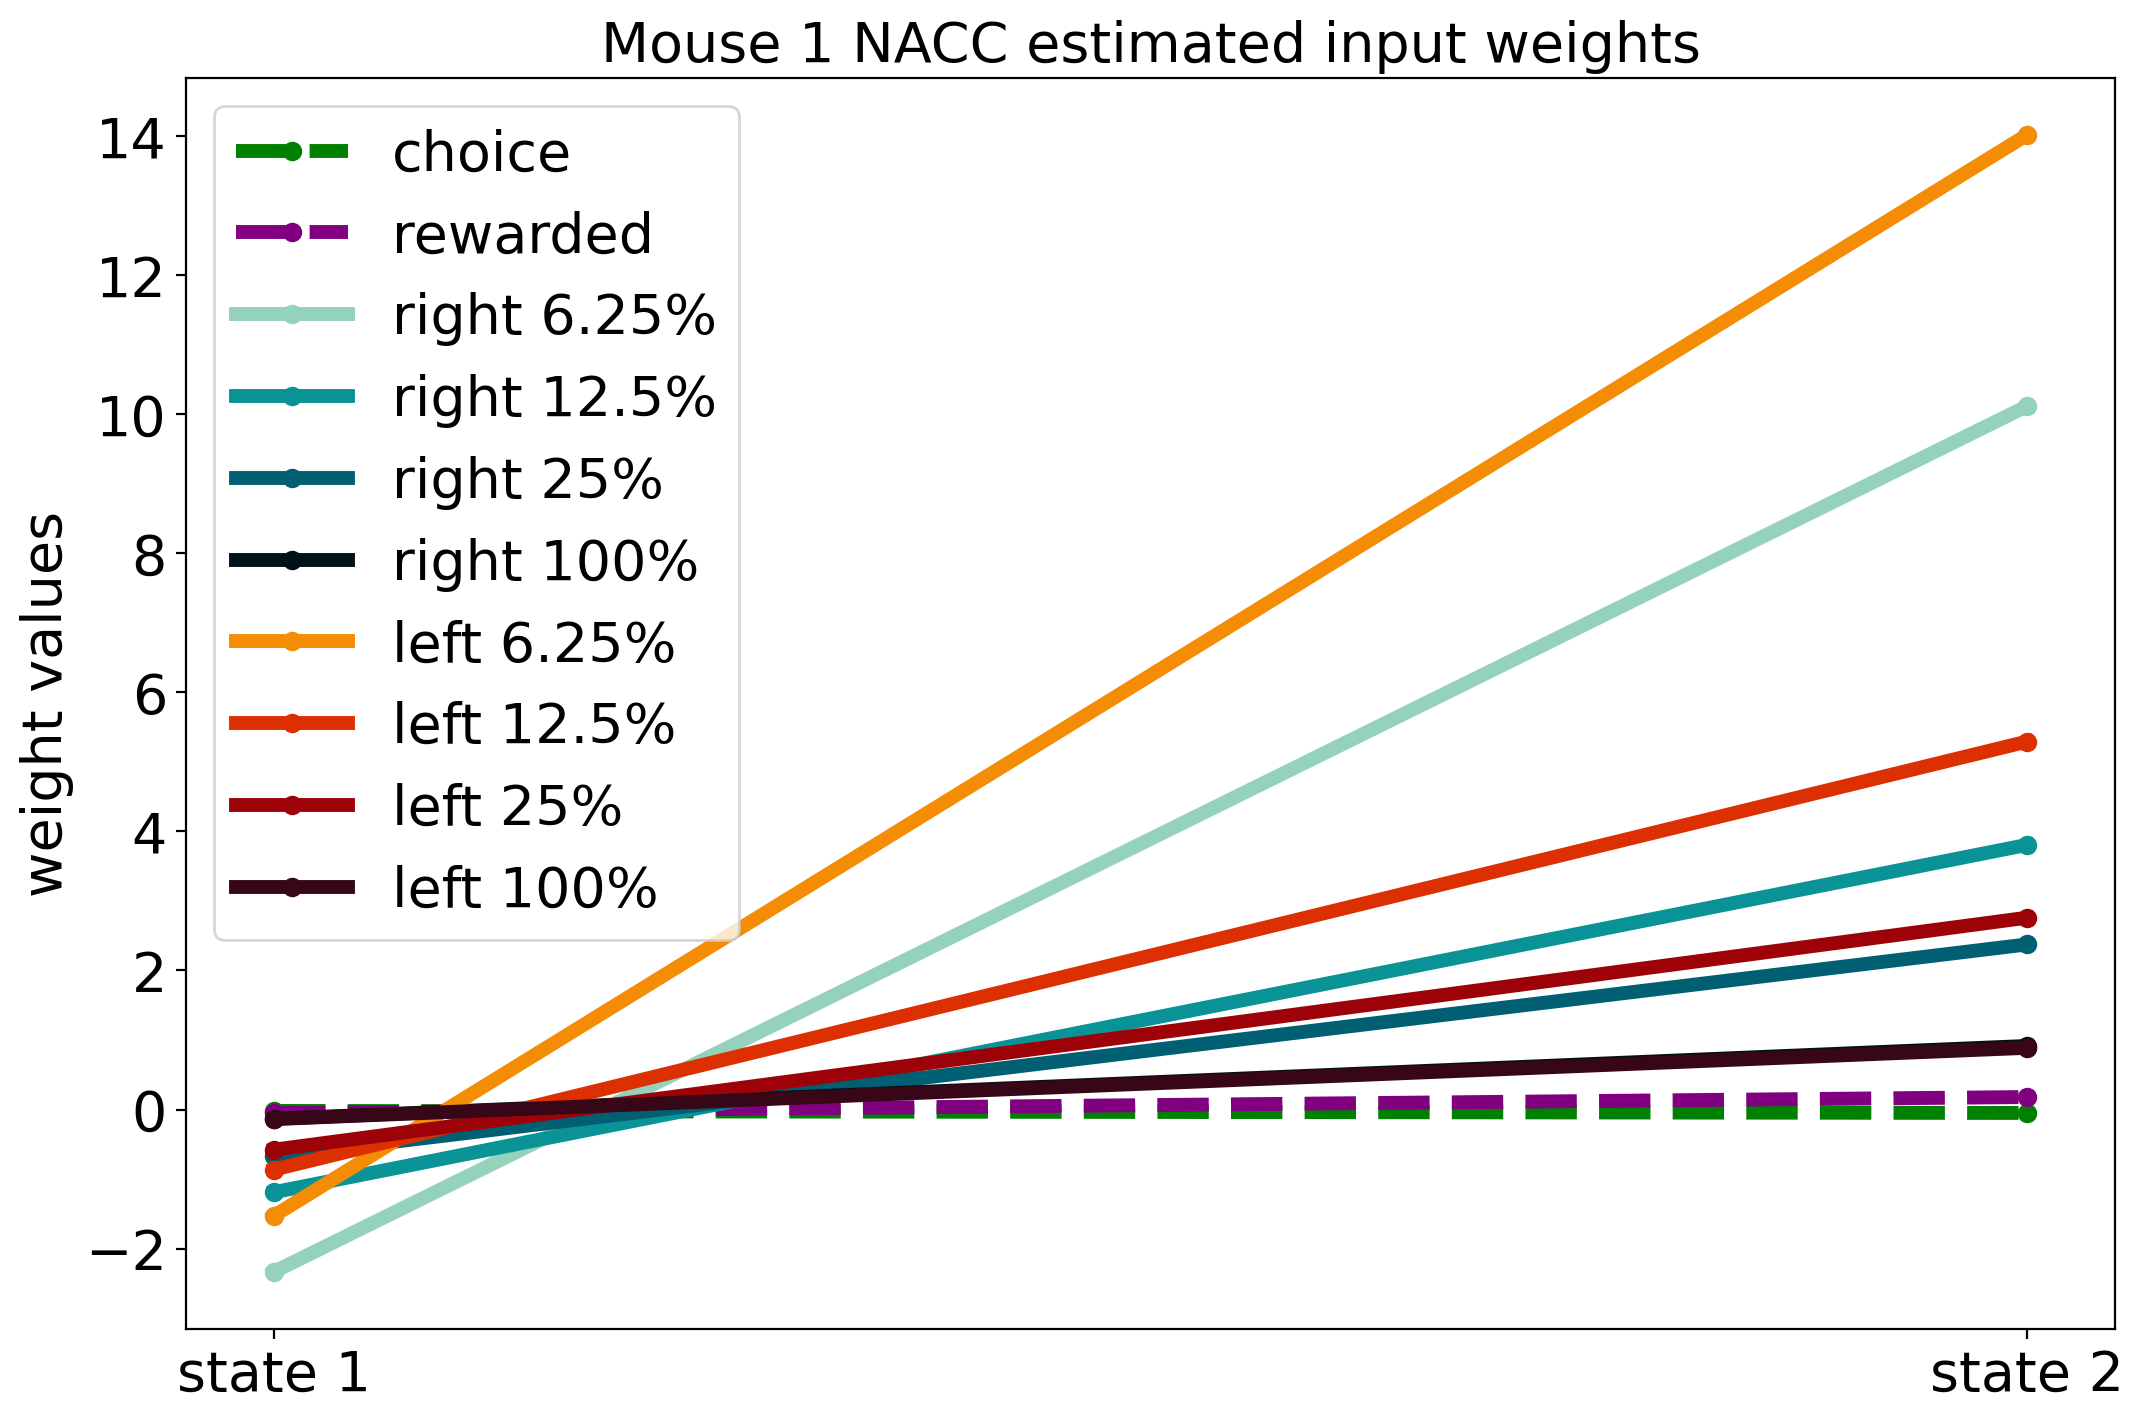
\includegraphics[width=10cm]{stim_images/2state_W.png}
 \caption{Estimated input weights by state for the 2-state model fit the neural data of stimulus presentation.}
\end{figure}
\noindent
The results of figure 3 above are interesting. In particular we see that states 1 and 2 can be interpreted as engaged and dis-engaged respectfully. This is due to the fact that the model estimates larger weights for the neural responses at stimulus presentation only in state 2. Further more, the lower the contrast level the more difficult it is for the animal to see the stimulus. That the most difficult contrast to see, both on the left and right side of the screen have the largest weights is intuitive. In a sense more "importance" must be placed on stimulus that are more difficult to see, but could lead to a correct decision being made. In contrast, the easiest stimuli to see (largest contrast) have the smallest weights. We note that this replicates results previously found in mice [2, 3]. While figure 3 is convincing for the argument of an engaged and dis-engaged state, it leads to a prediction about what the estimated state probabilities will look like in this model. We recall that this data is gathered over periods of learning. Thus, if state 2 is in-fact an "engaged" state, then by inspecting the estimated state probabilities, we should at some point see a transition where state 2 becomes more probable, and this should occur later in training. This is what we see in figure 4.
\begin{figure}[H]
\centering
 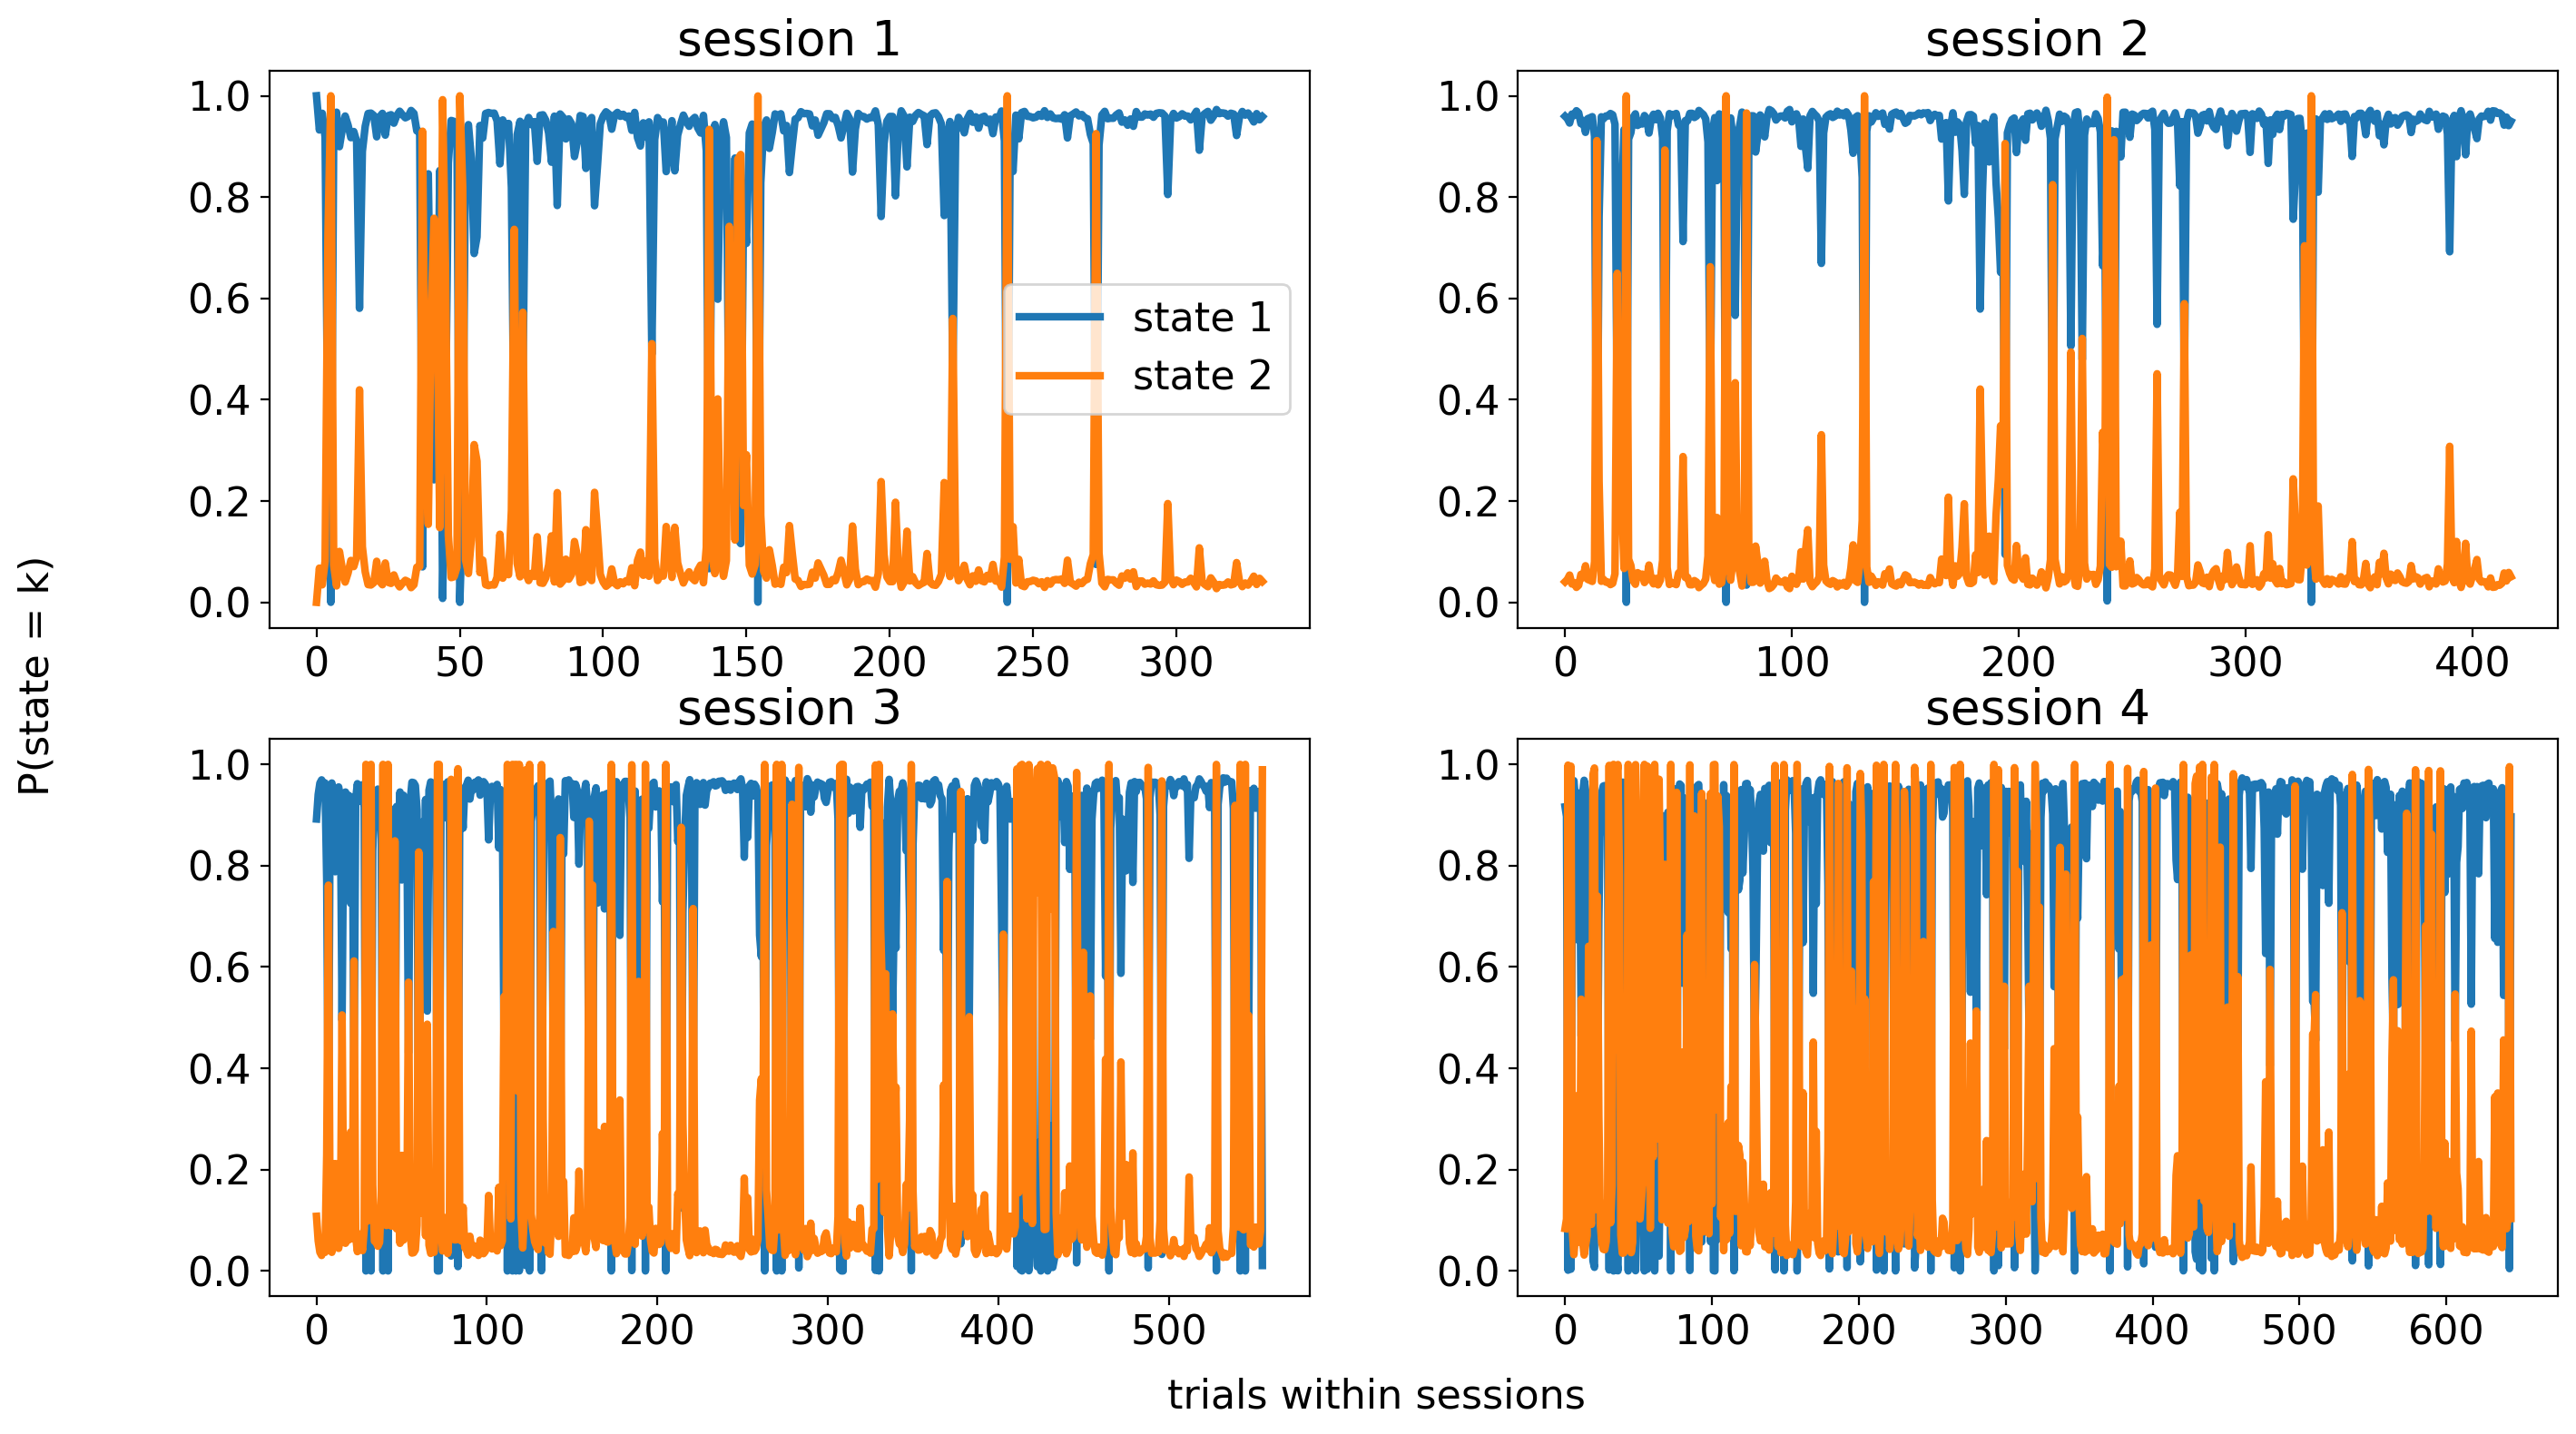
\includegraphics[width=14cm]{stim_images/first_4_days_2state_gammas.png}
 \caption{Estimated state probabilities. The first 4 sessions of training are displayed. We note that, as the animal becomes more familiar with the task, in terms of time, state 2 (the engaged state) becomes more and more probable. }
\end{figure}

Finally we investigate the transition matrix for the 2-state model and the neural data at stimulus presentation. The transition matrix of figure 5 conveys how likely the animal is to move to a different state. Keeping the interpretation of state 1 as the dis-engaged and state 2 the engaged state, we see that if the animal is in the dis-engaged state, it has high probability of remaining in that state. From this dis-engaged state however, it has a relatively good chance of going into the engaged state. On the other hand, the animal is less likely to transition from the engaged state to the dis-engaged state. And has a modest chance of remaining in the engaged state. 

\begin{figure}[H]
\centering
 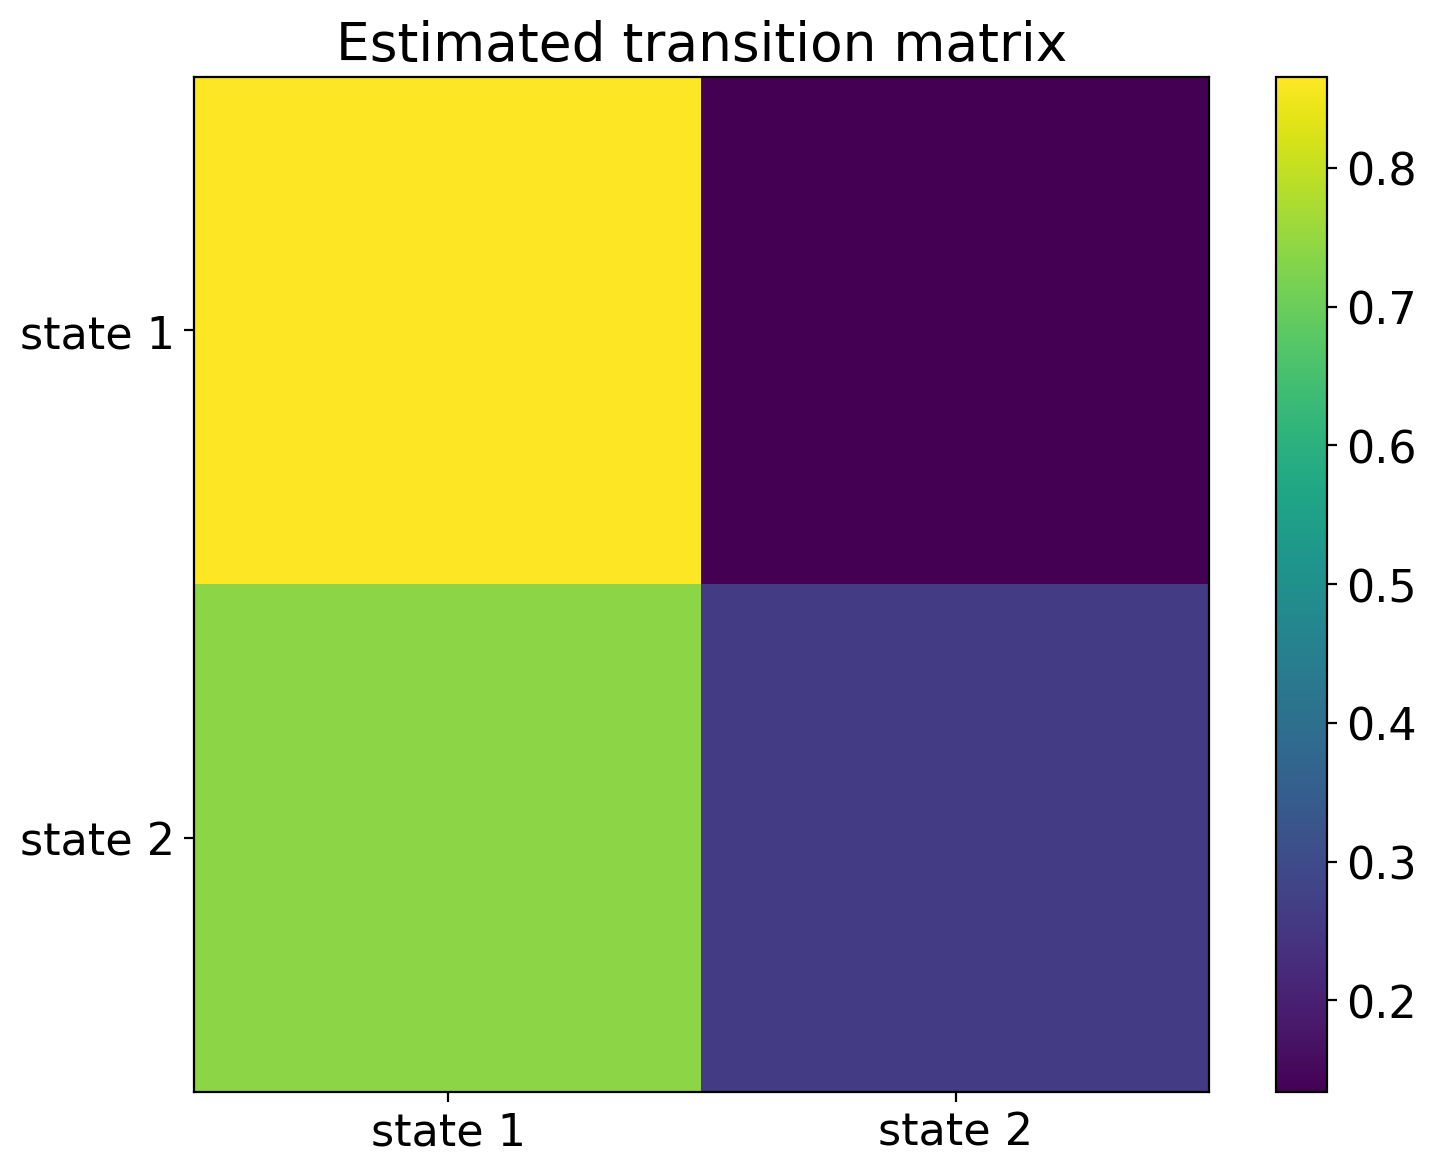
\includegraphics[width=8cm]{stim_images/trans_mat_2state.png}
 \caption{Estimated state transition matrix in the 2-state model for the neural data corresponding to stimulus presentation.}
\end{figure}

We recall that in the comparison of the log-likelihoods, the 3-state model provided a better fit to the data at feedback time. We now look at the weights for the 3-state model using the neural data at feedback delivery. We predict that in this model, we will see the largest coefficients estimated for the inputs corresponding to reward. This is in fact what we see in figure 6. In addition, we see that in the 3rd state we estimate the largest coefficient for reward. In this state the coefficients for the stimulus are also largest. This is intuitive, as being able to take into account the stimulus is a necessary condition for making the correct choice, and thus being rewarded. Moreover, the stimulus at the highest contrast and consequently easiest to see are represented the most in terms of magnitude in the coefficients which makes sense as they more frequently lead to reward. 

\begin{figure}[H]
\centering
 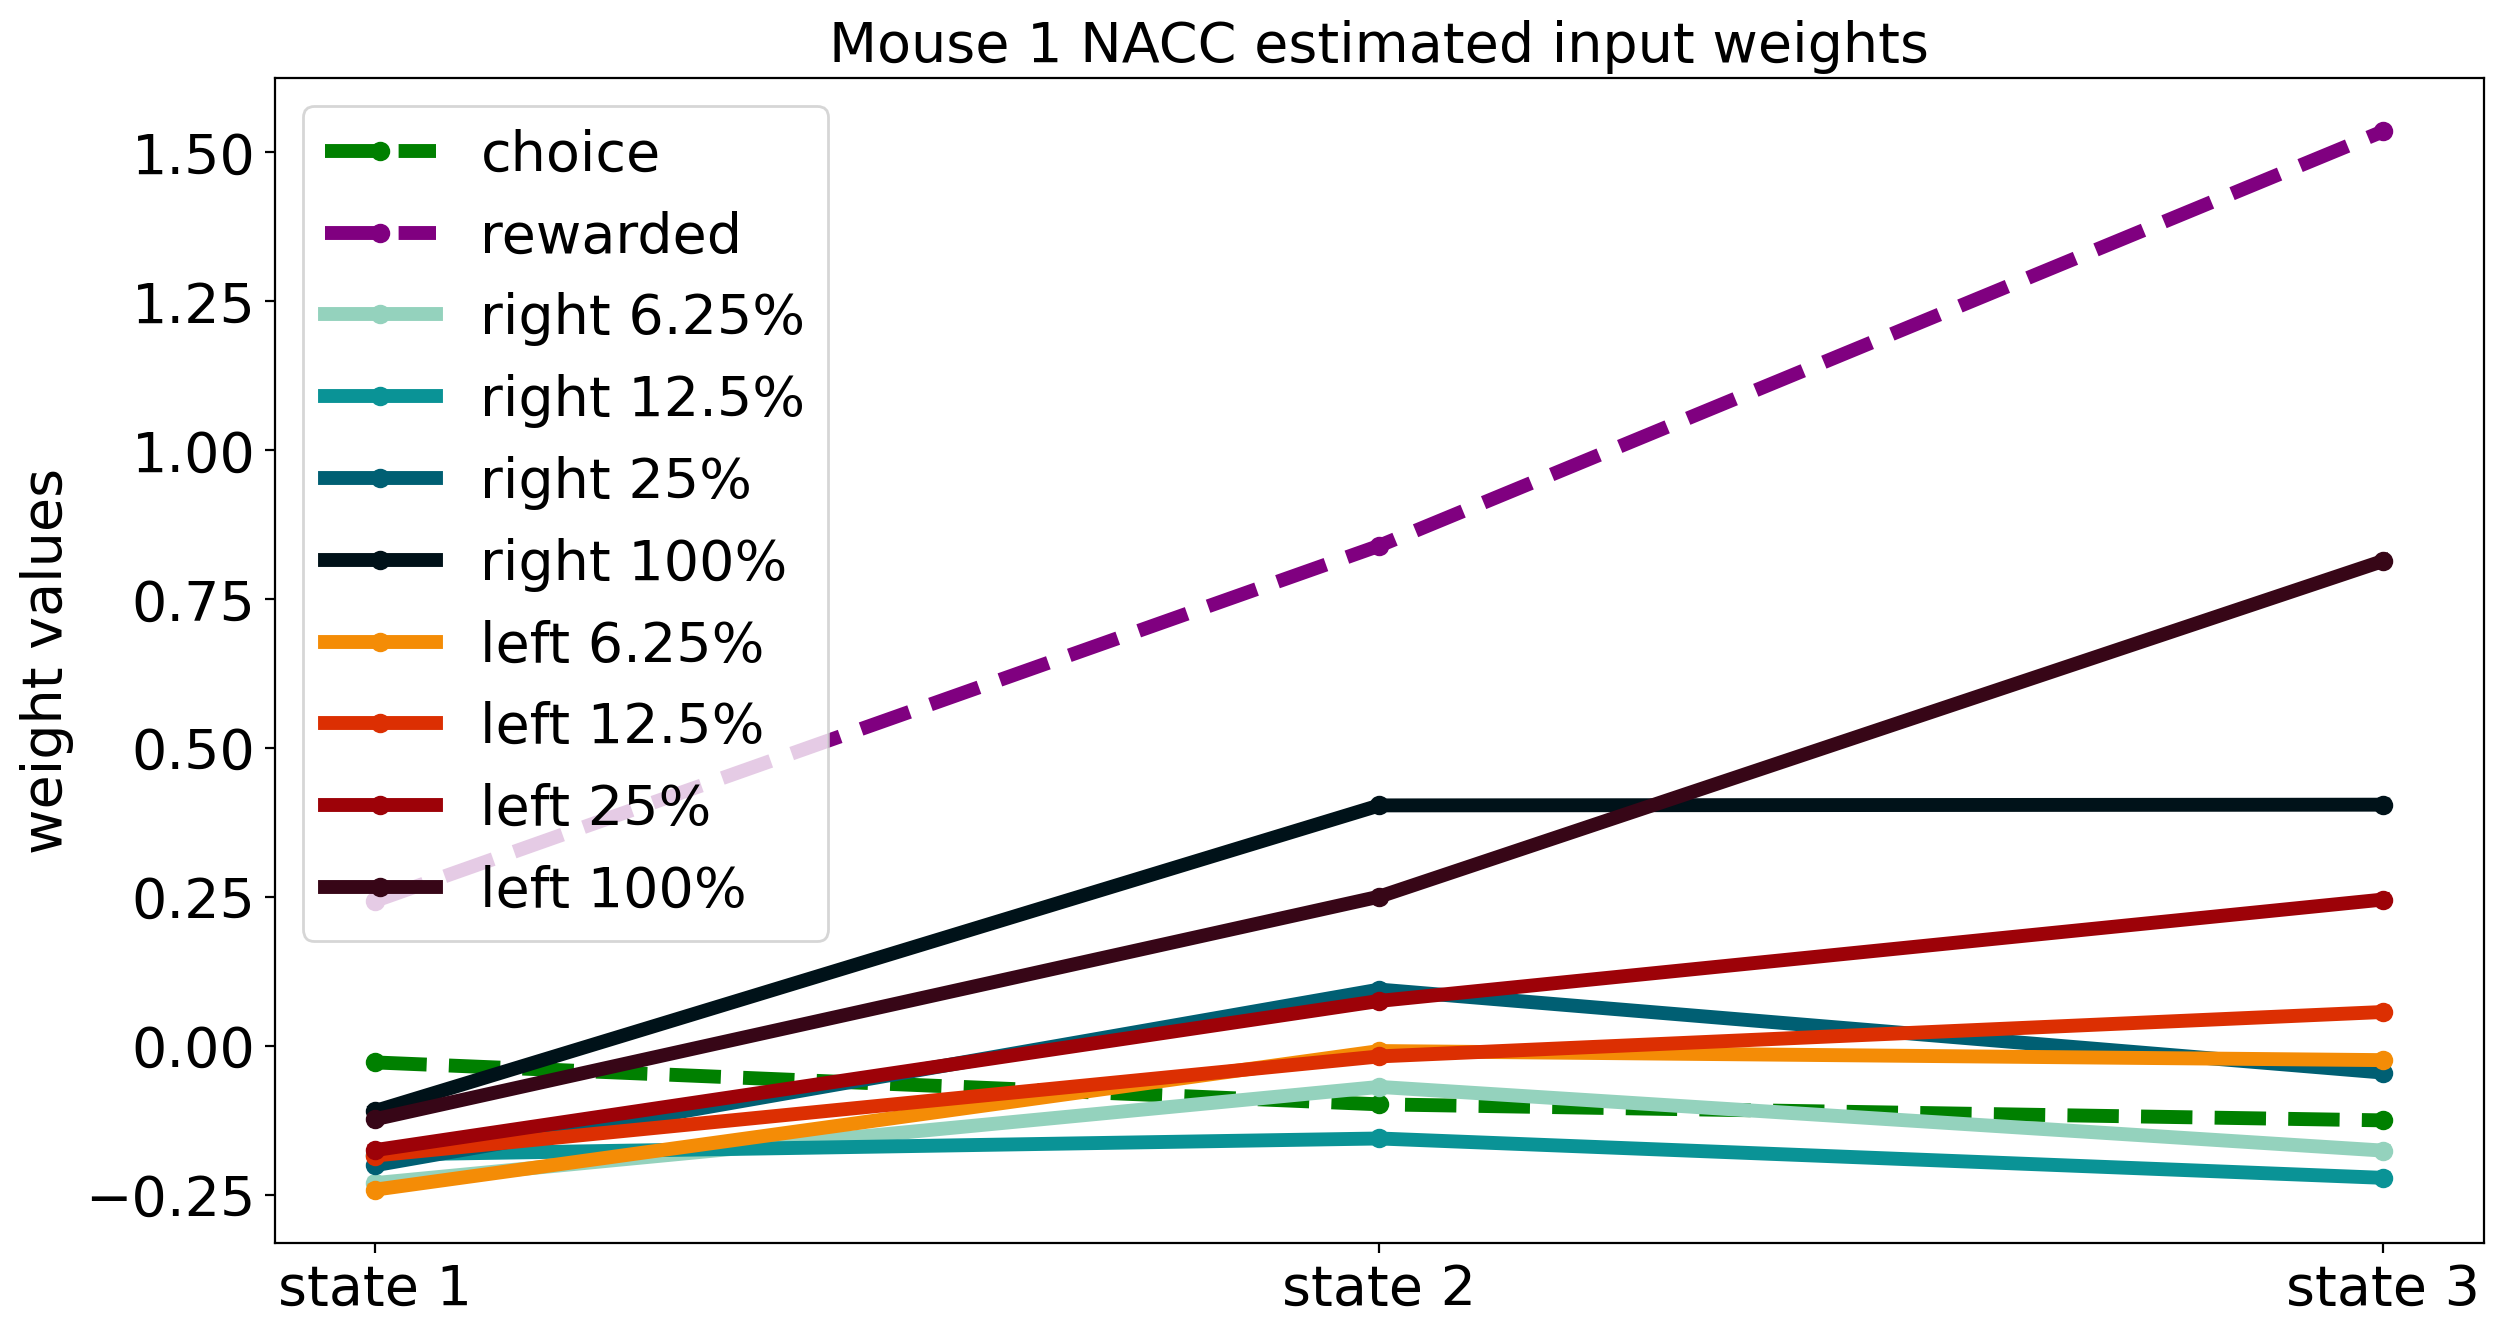
\includegraphics[width=12cm]{feed_images/W_states__feedback_3fip29.png}
 \caption{Estimated input weights for the 3-state model, using the neural data at feedback / reward delivery. }
\end{figure}

\section{Discussion \& Future work}
In this project we applied a variant of the Input Output Hidden Markov Model to neural data. Hidden Markov models are valuable for Neuroscience because the design of the model mimics an intrinsic fact about the experimental design. Often in Neuroscience researchers are working with model species such as mice. Unlike humans, we have no way of directly querying what the mice think via language. Thus at any time in point, the mice can be in an internal state that influences their performance on the task, and thus the results of the study. By attempting to chunk the data according to the states estimated in models such as Hidden Markov Models, we may be able to more accurately describe both the neural and behavioral responses. For example, as we saw in the results above, the mice might be in a dis-engaged state. In this state the reward may be of little interest to the mouse. In sub-fields such as decision making neuroscience, unintentionally mixing brain signals that come from engaged and dis-engaged states can greatly confuse the experimental results. 

The results outlined above are promising but incomplete. We only applied a variant of the model that uses neural data, however during learning both behavioral and neural data is collected. Thus in future work we hope to expand on this model with an IO-HMM whose latent variables have two-emissions per time point. This is a more natural abstraction of the interplay between the brain, behavior, and the task. Building on this, we want to add input driven transitions to the model. In the current model, we only have input driven emissions. Having these input driven variables is of great important as they add an additional layer of accuracy to the abstraction of the HMM. Specifically, the mice are shown stimuli, they make choice, and are rewarded. Each of these factors effects their subsequent behavior and the neural data acquired. Thus having both input driven transitions and emissions as in done in [1] will be an important next step. Another addition to this work will be figuring out how to deal with the numerical challenges of using non-averaged data. The current data used consisted of averages within trials of the periods for stimulus presentation and feedback delivery. This was necessary as the non-averaged data amounted to roughly 10 million samples by 1000 features, and the current model simply could not fit this data due to numerical and memory constraints. Figuring out how to work with this richer dataset will allow for a much cleaner interpretation of the results. Lastly, a GLM is a relatively simple model to explain the complexity of a neural response. For this reason we would like to leverage the composition of neural networks with graphical models such as HMM, as done in [5]. 








\section*{References} 

[1]. Calhoun AJ, Pillow JW,  Murthy M. (2019). Unsupervised identification of the internal states that shape natural behavior. Nature Neuroscience 22:2040-20149.

\bigskip
\noindent
[2]. Ashwood ZC, Roy NA, Stone, IR, The International Brain Laboratory, Urai AE, Churchland, AK, Pouget A, Pillow JW (2022).
Mice alternate between discrete strategies during perceptual decision-making. Nature Neuroscience 25 (2): 201–212.

\bigskip
\noindent
[3]. Bolkan SS*, Stone IR*, Pinto L, Ashwood ZC, Garcia JMI, Herman AL, Singh P, Bandi A, Cox J, Zimmerman CA, Cho JR, Engelhard B, Pillow JW, Witten IB (2022). Strong and opponent contributions of dorsomedial striatal pathways to behavior depends on cognitive demands and task strategy. Nature Neuroscience 25 (3): 345–357.

\bigskip
\noindent
[4]. Input-Output HMMs for sequence processing. 1996 Y Bengio, P Frasconi. IEEE

\bigskip
\noindent
[5]. Johnson, M.J., Duvenaud, D., Wiltschko, A.B., Datta, S.R., and Adams, R.P. (2016). Composing graphical models with neural networks for structured representations and fast inference. In 30th Conference on Neural Information Processing Systems (NeurIPS)




\end{document}